{\color{gray}\hrule}
\begin{center}
\section{Setting up the simulation}
\textbf{Processing SELECT trial data and estimating caloric requirements}
\bigskip
\end{center}
{\color{gray}\hrule}

\subsection{Data from SELECT Trial}
To accurately model weight loss across different BMI categories, we analyzed the SELECT trial data \cite{Ryan2024} using a systematic approach to account for treatment adherence and placebo effects. Our goal was to determine the true treatment effect of semaglutide assuming perfect adherence.

The analysis incorporated three key components from the trial:
\begin{itemize}
    \item Estimated Treatment Differences (ETD) for each BMI category
    \item Placebo group weight loss (-1.5\% at 4 years)
    \item Adherence adjustment (+1.5\% based on first on-treatment analysis)
\end{itemize}

The adherence-adjusted weight loss was calculated using:
\begin{equation}
    \text{Adjusted Weight Loss} = (\text{ETD} + \text{Placebo Loss}) + 1.5\%
\end{equation}

\begin{table}[h]
\centering
\begin{tabular}{|l|c|c|c|c|}
\hline
\textbf{BMI Group} & \textbf{ETD (\%)} & \textbf{Placebo (\%)} & \textbf{Initial (\%)} & \textbf{Adjusted (\%)} \\
\hline
BMI $<$30 & -7.52 & -1.5 & -9.02 & -10.52 \\
BMI 30-35 & -8.79 & -1.5 & -10.29 & -11.79 \\
BMI 35-40 & -9.01 & -1.5 & -10.51 & -12.01 \\
BMI $\geq$40 & -9.23 & -1.5 & -10.73 & -12.23 \\
\hline
\end{tabular}
\caption{Weight loss percentages by BMI category, adjusted for adherence}
\end{table}

\subsection{Adjusting for our Model}
To translate these findings into our simulation framework, we first converted BMI categories to target weights using our model subject's height (1.8m). We then performed a binary search to determine both the pre-treatment caloric intake needed to reach each BMI category and the treatment-phase intake required to achieve the observed weight loss.

This process yielded the following caloric requirements:

\begin{table}[!htb]
\centering
\begin{tabular}{|l|c|c|c|c|c|c|}
\hline
\textbf{BMI Group} & \textbf{Initial} & \textbf{Initial} & \textbf{Final} & \textbf{Final} & \textbf{Weight} \\
& \textbf{Weight (kg)} & \textbf{Calories} & \textbf{Weight (kg)} & \textbf{Calories} & \textbf{Change (\%)} \\
\hline
BMI $<$30 & 76.2 & 2,353 & 68.2 & 2,098 & -10.5 \\
BMI 30-35 & 88.5 & 2,730 & 78.0 & 2,401 & -11.8 \\
BMI 35-40 & 102.1 & 3,152 & 89.8 & 2,766 & -12.0 \\
BMI $\geq$40 & 114.3 & 3,530 & 100.4 & 3,091 & -12.2 \\
\hline
\end{tabular}
\caption{SELECT Trial Analysis Results (Pre-treatment: 7 years, Treatment: 4 years)}
\end{table}

When we simulate the model with these caloric requirements, we get the following weight trajectories:

\begin{figure}[!htb]
\centering
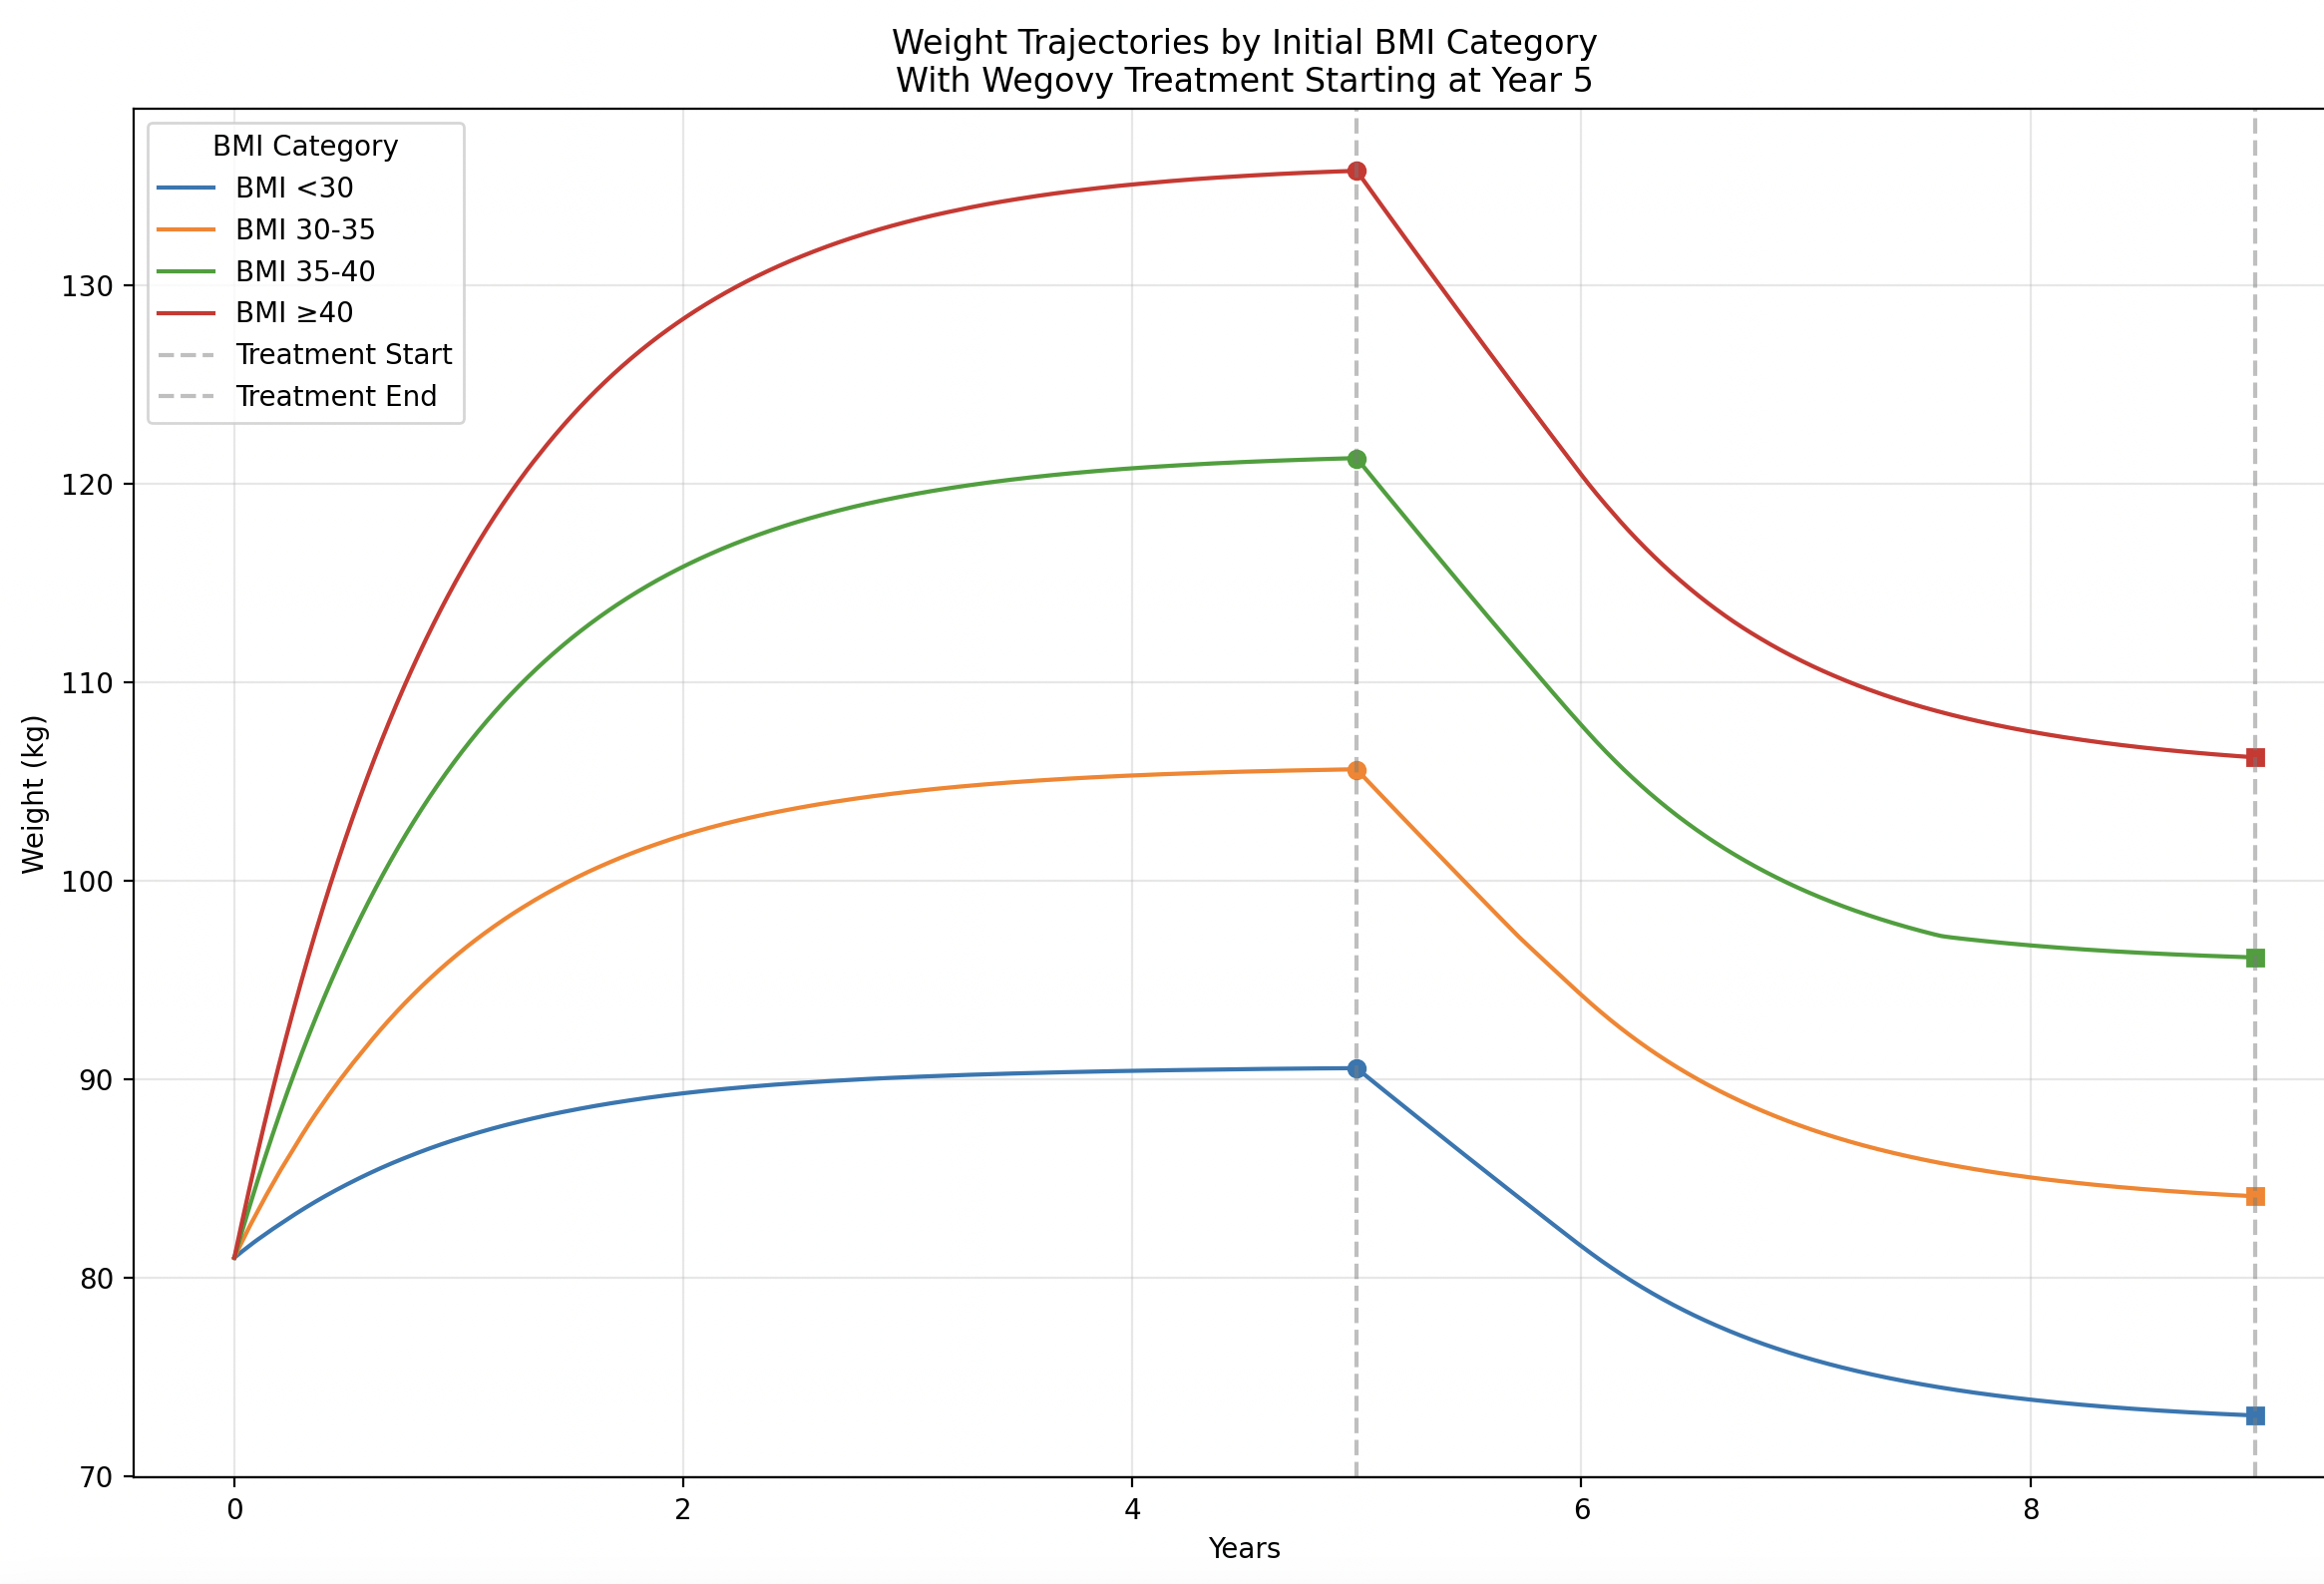
\includegraphics[width=0.8\textwidth]{images/wegovy_weights_plot.png}
\caption{Simulated weight trajectories by BMI category showing pre-treatment weight gain and subsequent Wegovy treatment response}
\label{fig:wegovy_weights}
\end{figure}

This matched the observed weight loss in the SELECT trial, indicating that our caloric requirements were accurate.

\subsection{Creating the Ramp-Up Function}
To accurately model the gradual onset of Wegovy's appetite-suppressing effects, we implemented a ramp-up function that simulates the typical clinical titration schedule. The function gradually increases the medication's effect over time, which better reflects real-world patient experiences and helps avoid sudden caloric restrictions.

\begin{equation}
    \text{Ramp Factor} = \min\left(\frac{t - t_{\text{start}}}{t_{\text{ramp}}}, 1\right)
\end{equation}

where:
\begin{itemize}
    \item $t_{\text{start}}$ = 1825 days (5-year pre-treatment period)
    \item $t_{\text{ramp}}$ = 60 days (2-month ramp-up duration)
\end{itemize}

The caloric adjustment is then applied using:
\begin{equation}
    \text{Caloric Reduction} = \text{Target Reduction} \times \text{Ramp Factor}
\end{equation}

This gradual approach ensures that:
\begin{itemize}
    \item The treatment effect increases linearly over the first year
    \item The full effect is achieved only after complete titration
    \item The simulation better matches clinical observations of weight loss patterns
\end{itemize}


